\begin{figure*}[htbp]
	\centering
	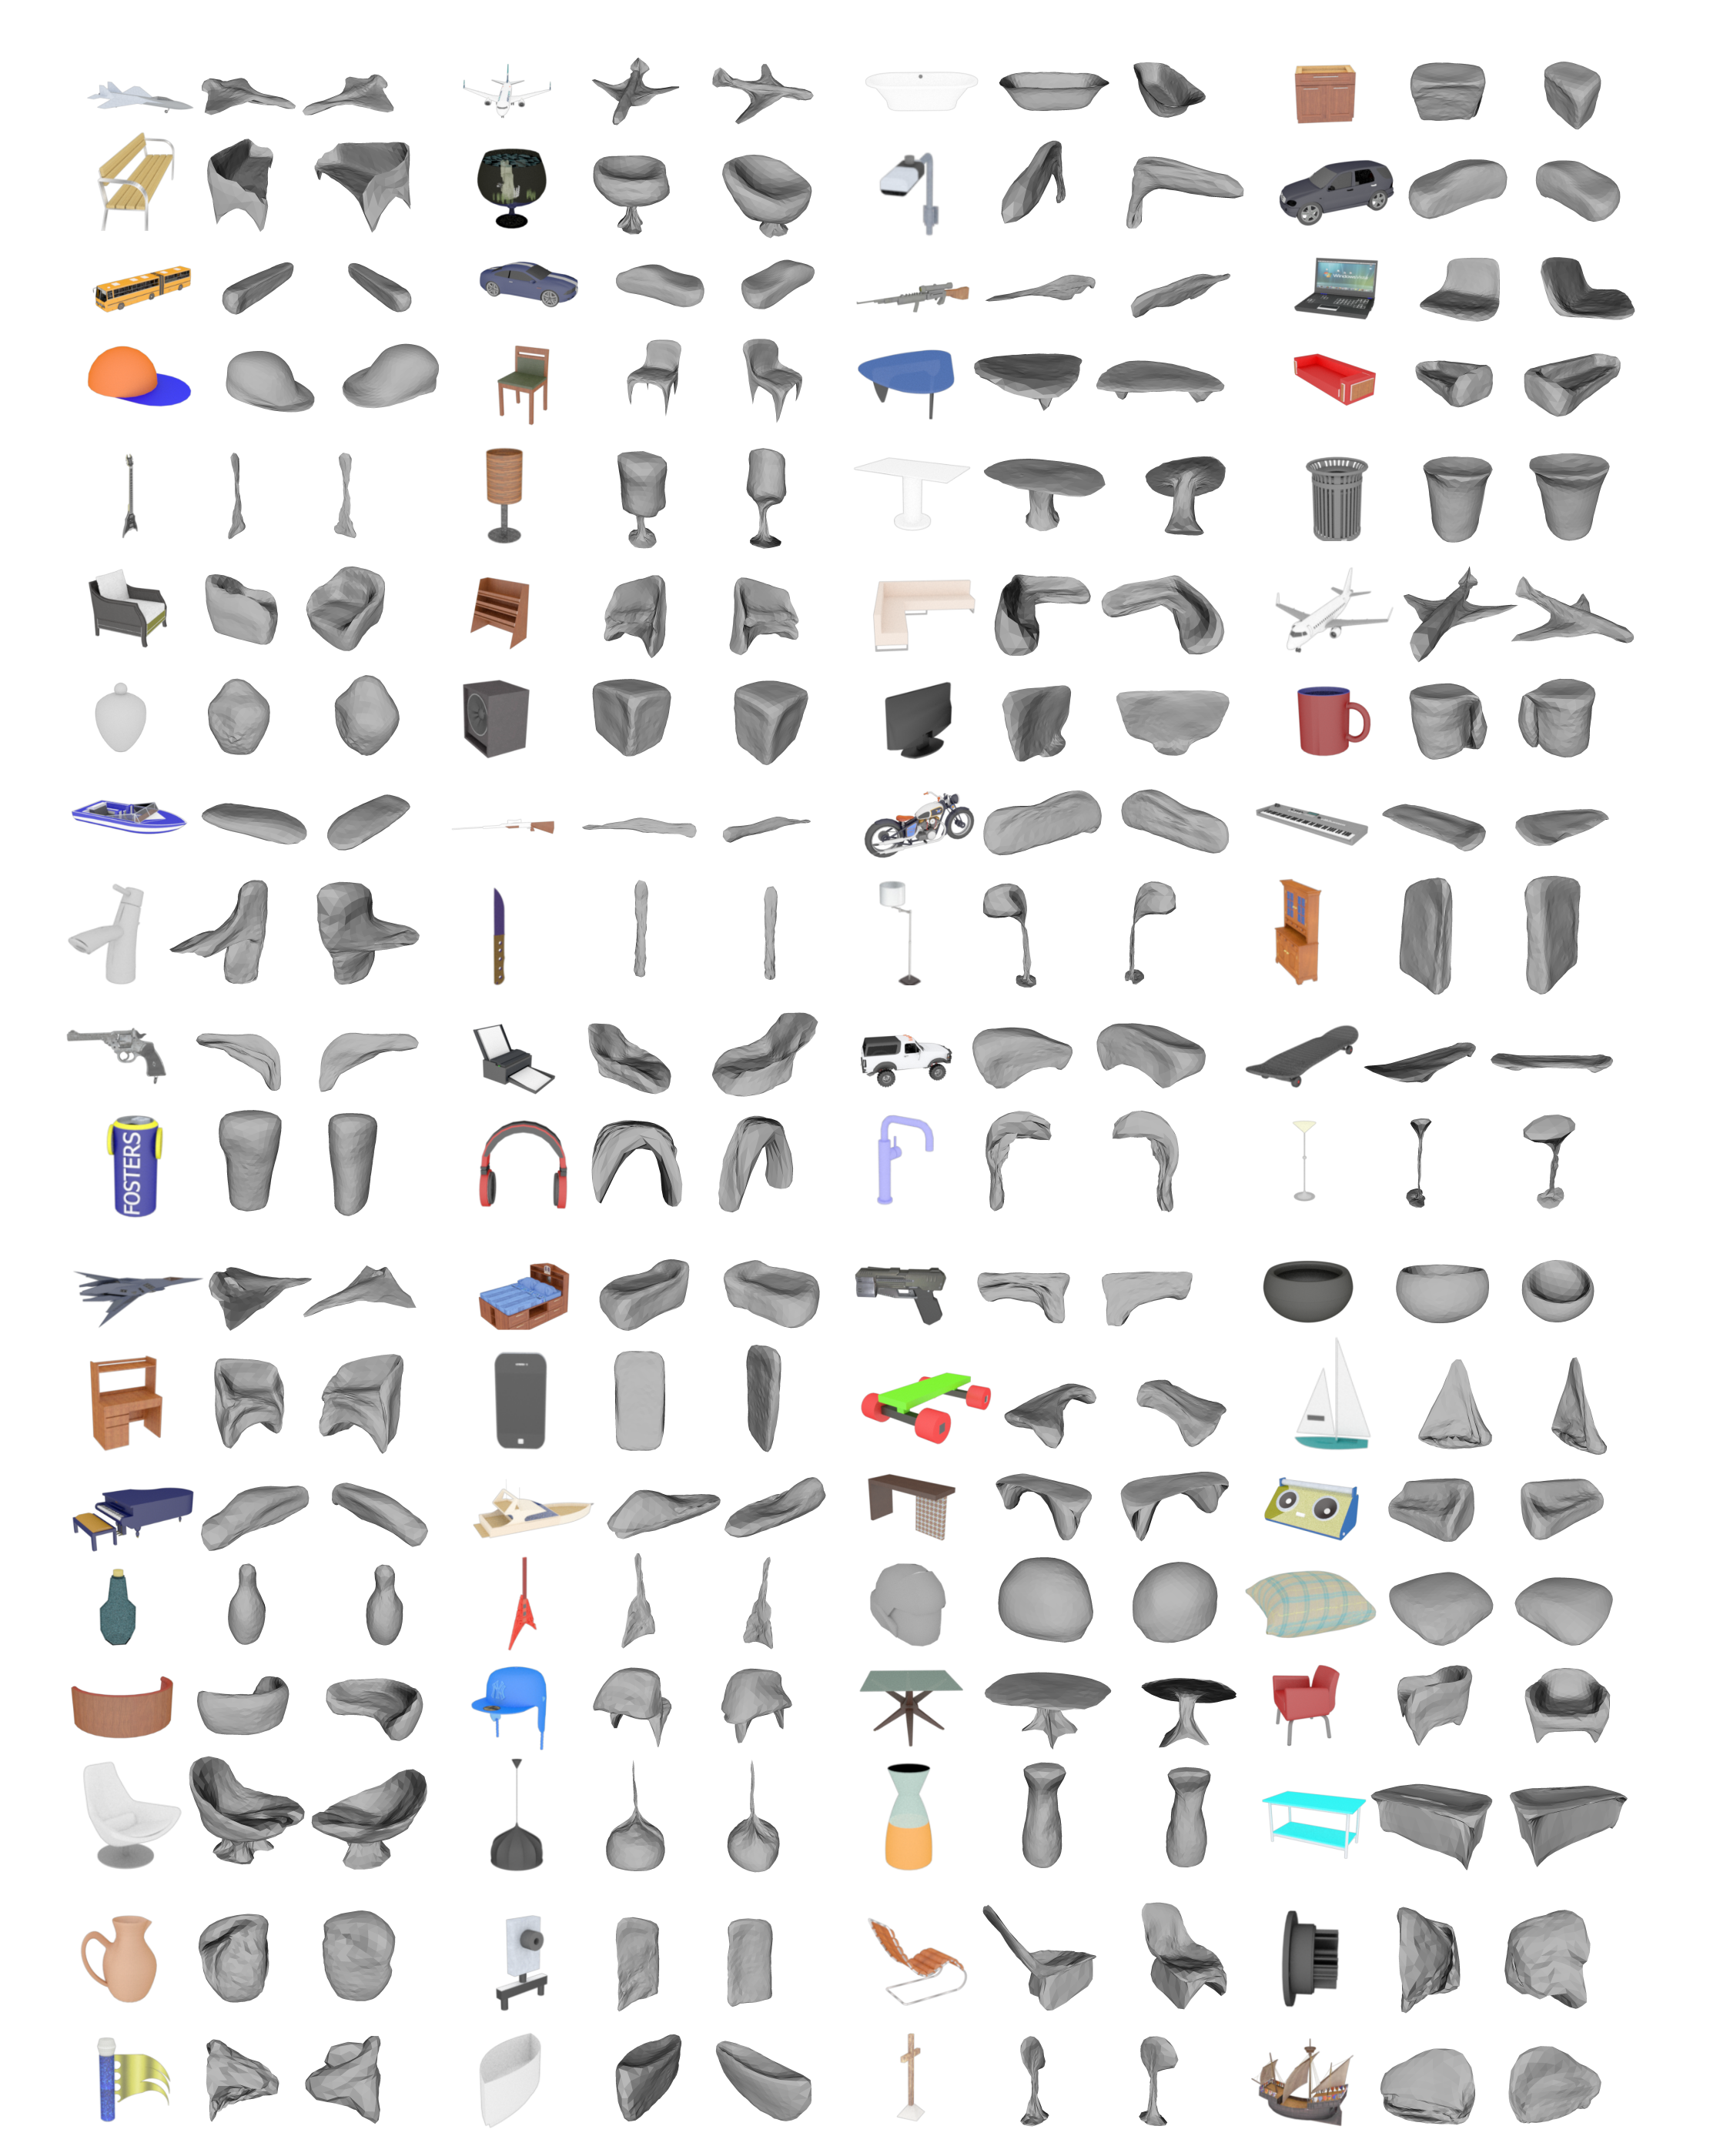
\includegraphics[width=\linewidth]{img/more_res/res}
	\caption{More visual results randomly picked from testing data}
	\label{fig:more_res}
\end{figure*}
\section{Experiments}
In this section, we evaluate our network through a series of experiments.
\subsection{Experimental setup}
%%===data===%%
We train and evaluate our models on the ShapeNet\cite{shapenetdata}. Specifically, we use the ShapeNetCore55.v2 which contains over 50k of
manually created and cleaned 3D CAD models in 55 category.
The images for training
and testing are rendered in random angles to provide synthetic training data for the model. In total,
51,856 shape models are covered. For the training/validation/testing split, we follow the CSV file provided by the ShapeNet website and resulted in 36,622/5,110/10,124 shapes. The 3D CAD objects are
stored as meshes, we re-sample the meshes into point sets. In order to capture only the shape surface, we uses the code from \cite{ocnn} and execute ``virtual scan" for the re-sampling.
\subsection{Comparing to state-of-the-art}
In this subsection, we compare our approach with the state-of-the-art point set generation network (PSGN)\cite{PSGN}. In Table~\ref{tab:seg}, we compare the our approach with PSGN\cite{PSGN} in quantitative evaluation over all category of objects in testing data. The results shows that our approach achieves over all comparable performance with PSGN\cite{PSGN} under Chamfer distance and present evidently better performance under Earth mover distance. 
In Figure~\ref{fig:res}, we compare the visual results of our framework (ParamNet) and PSGN\cite{PSGN}. In Figure~\ref{fig:res}, we also show mesh generated by ball-pivoting\cite{ballpivot} from the output point set of PSGN\cite{PSGN}. These visual results shows that it is difficult to recover continuous surface from the point set generated by PSGN\cite{PSGN} since it does not explicitly consider local structure of the generated surface, while our method can generate continuous surface for various objects.
\begin{table*}
	\caption{Comparison with point set generation network\cite{PSGN}}
	\label{tab:seg}
	\centering
	\begin{tabular}{c c c c c c}
		\multirow{2}{*}{Category} & \multirow{2}{*}{Category id} & \multicolumn{2}{c}{Chamfer} & \multicolumn{2}{c}{EMD}\\ \cmidrule(lr){3-4} \cmidrule(lr){5-6}
		&	& ParamNet & PSGN\cite{PSGN}       & ParamNet & PSGN\cite{PSGN}\\
		\hline
		aircraft & 02691156 & 0.068 & 0.058 & 0.248 & 0.502 \\   
		dustbin & 02747177 & 0.162 & 0.166 & 0.425 & 1.947 \\
		bag & 02773838  & 0.398 & 0.453 & 0.921 & 3.258 \\
		basket & 02801938 & 0.861 & 0.708 & 1.545 & 2.186 \\
		bathtub & 02808440 & 0.072 & 0.070 & 0.175 & 0.472 \\
		bench & 02828884 & 0.063 & 0.063 & 0.239 & 0.641 \\
		bed & 02818832 & 0.362 & 0.291 & 0.865 & 1.523 \\
		birdhouse & 02843684 & 0.855 & 0.624 & 1.972 & 4.332 \\
		shelf & 02871439 & 0.100 & 0.081 & 0.407 & 1.475 \\
		bottle & 02876657 & 0.075 & 0.084 & 0.289 & 1.340 \\
		bowl & 02880940 & 0.726 & 0.423 & 0.954 & 1.646 \\
		bus & 02924116 & 0.035 & 0.036 & 0.306 & 0.602\\
		dresser & 02933112 & 0.082 & 0.078 & 0.168 & 0.799 \\
		camera & 02942699 & 0.818 & 0.752 & 1.889 & 3.124 \\
		can & 02946921 & 0.165 & 0.180 & 0.778 & 4.247 \\
		cap & 02954340 & 1.466 & 2.738 & 2.795 & 3.559 \\
		car & 02958343 & 0.051 & 0.047 & 0.176 & 0.399 \\
		cellphone & 02992529,04401088 & 0.143,0.039 & 0.128,0.030& 0.965,0.150 & 7.583,0.974\\
		chair & 03001627 & 0.042 & 0.038 & 0.117 & 0.605 \\
		clock & 03046257 & 0.152 & 0.119 & 0.387 & 1.194 \\
		keyboard & 03085013 & 0.450 & 0.456 & 1.470 & 2.626\\
		dishwasher & 03207941 & 0.204 & 0.236 & 0.501 & 2.975 \\
		monitor & 03211117 & 0.079 & 0.067 & 0.224 & 0.811\\
		headphone & 03261776 & 0.738 & 0.590 & 3.906 & 4.499 \\
		hydrant & 03325088 & 0.177 & 0.151 & 0.748 & 1.123 \\
		file cabinet& 03337140 & 0.121 & 0.113 & 0.325 & 1.949 \\
		guitar & 03467517 & 0.014 & 0.015 & 0.278 & 1.234 \\
		helmet & 03513137 & 0.789 & 1.199 & 1.693 & 2.387 \\
		vase & 03593526 & 0.088 & 0.082 & 0.305 & 1.244 \\
		knife & 03624134 & 0.034  & 0.029 & 0.280 & 2.089 \\
		lamp & 03636649 & 0.089 & 0.084 & 0.503 & 0.869\\
		laptop & 03642806 & 0.174 & 0.154 & 0.537 & 1.262 \\
		speaker & 03691459 & 0.125 & 0.117 & 0.315 & 0.806 \\
		mailbox & 03710193 & 0.258 & 0.252 & 1.245 & 4.337 \\
		mike & 03759954 & 1.599 & 1.301 & 3.149 & 6.842 \\
		microwave & 03761084 & 0.305 & 0.302 & 0.675 & 2.647 \\
		motorcycle & 03790512 & 0.153 & 0.139 & 0.522 & 1.495\\
		mug & 03797390 & 0.269 & 0.188 & 0.481 & 1.568 \\
		piano & 03928116 & 0.234 & 0.227 & 0.693 & 1.587 \\
		pillow & 03938244 & 0.614 & 0.526 & 0.996 & 2.101 \\
		handgun & 03948459,04090263 & 0.372,0.049 & 0.309,0.049 & 1.158,0.304 & 2.369,0.790 \\
		planter & 03991062 & 0.124 & 0.139 & 0.301 & 0.839 \\
		printer & 04004475 & 0.500 & 0.413 & 1.064 & 1.716 \\
		remote & 04074963 & 0.106 & 0.105 & 0.846 & 5.940 \\
		missile & 04099429 & 0.220 & 0.187 & 1.874 & 4.113 \\
		skateboard & 04225987 & 0.369 & 0.295 & 1.696 & 2.232 \\
		sofa & 04256520 & 0.051 & 0.052 & 0.172 & 0.321 \\
		stove & 04330267 & 0.184 & 0.214 & 0.488 & 1.528 \\
		table & 04379243 & 0.077 & 0.075 & 0.271 & 0.537 \\
		tower & 04460130 & 0.620 & 0.735 & 1.714 & 3.812 \\
		train & 04468005 & 0.129 & 0.122 & 0.638 & 1.140 \\
		ship  & 04530566 & 0.067 & 0.057 & 0.273 & 0.620 \\
		washer &  04554684 & 0.205 & 0.203 & 0.482 & 1.957 \\
		\hline
		mean   &     -     & 0.297 & 0.298 & 0.834 & 2.086
	\end{tabular}
\end{table*}
\subsection{Ablation study}
In this subsection, we do ablation study to investigate the functionality of each components in our framework. The evaluation are shown in Table~\ref{tab:ablation} and Table~\ref{tab:pointnet}. Some visual result for the ablation study are shown in Figure~\ref{fig:abl}. Now we discuss these results as follows:

\noindent\textbf{Laplacian smooth}
The Laplacian smooth force the output surface to have more regular local structure. When Laplacian smooth is removed, the output surface become much more rough as shown in Figure \ref{fig:abl} under the column of ``-Laplacian smooth".

\noindent\textbf{Initialization}
The initialization step reset the network to a state that output surface without self-intersection. As shown in Figure~\ref{fig:abl} under the column of ``-Initialization",  severe triangle flipping and self-intersection happens when the initialization training is skipped.

\noindent\textbf{Edge length regularization}
The edge length regularization term in the loss is designed to discourage over stretched triangles by minimizing the variance of edge length. According to our observation, when edge length regularization term is removed from the loss, the network tend to produce mesh that has  more large triangles as shown by the airplane example in Figure~\ref{fig:abl} under column ``-Edge length regularization ". Without such suppression for triangle over-stretching, the output become more easily to have self-intersection and triangle flipping as shown by the chair example in Figure~\ref{fig:abl} under column ``-Edge length regularization ".

\noindent\textbf{Normal loss}
The normal loss is designed to guide the learning by using the normal from groundtruth. According to our observation, the normal information is evidently useful to prevent some local self-intersection as highlighted by red rectangles in Figure~\ref{fig:abl}.

\noindent\textbf{Number of \textit{K}-neighbor PointNet}
The number of \textit{K}-neighbor PointNet is an important super parameter for our framework of networks. Based on the experiment results shown in Table~\ref{tab:pointnet}, we choose to use four \textit{K}-neighbor PointNet to construct the parameterization network, since the test error no longer diminishes when we use more (i.e. five). 

\subsection{Limitations and future work}
A major limitation for our framework is that it cannot handle the surface generation for objects that are not homotopy equivalent to sphere surface. This limitation arises from the design of our framework and is clearly shown in the cases in Figure~\ref{fig:fail1}. For this issue, we are planning to combine our framework with the method developed in \cite{assemble}. In this way, we can generate objects by several separate parts and therefore represent objects with more complicate topology.

Another limitation is that our semantic network failed to correctly infer the parameter for shape from the input image. Figure~\ref{fig:fail2} shows an example of such failure case. This limitation arises from the ambiguity in the 2D to 3D inference. For this issue, we are planning to try VAE method\cite{VAE} or min-of-n loss proposed by \cite{PSGN} to encode the ambiguity.  

